\chapter{Una aplicación de ejemplo}
Como \jj es una librería, no se la puede mostrar directamente en funcionamiento por lo que como parte del proyecto se planteo entregar una pequeña aplicación de ejemplo. Para mantener la simplicidad de la aplicación de ejemplo se decidió realizar la misma en dos partes. La primer parte es un \textit{script} que crea una base de datos, la segunda es una aplicacion un poco más compleja que muestra los datos que se crearon con el \textit{script} anterior.
\section{Creando la base de datos}
La primer parte de la aplicación de ejemplo es un mini-programa contenido en el fichero \verb=MakeDB.java= el cual contiene la clase \verb=MakeDB= que puede crear una base de datos y poblarla con datos al azar que se crean en base a una lista de nombres, direcciones, y domicilios. Los datos generados son para crear una base de datos que lleva el control de asistencia de una lista de alumnos de diferentes grados de un establecimiento educativo. La estructura de los datos generados en si no es importante, lo que interesa es demostrar como se puede usar \jj para poblar de datos una base de datos, además de crearla claro esta. EL mini-programa puede crear dicha base de datos en cualquiera de los motores que están siendo soportados por el proyecto, para ello es necesario cambiar una única linea de código. Si se observa el código fuente de esta primer parte se puede ver que se muestra una de las posibles formas de usar las clases que representan a \verb=CREATE TABLE, INSERT= y \verb=SELECT=.
\begin{lstlisting}[title=Código que debe alterarse para elegir el motor.]
// Constructor de la clase MakeDB
public MakeDB(String , String , String ) throws JDException {
	...
	// Debe elegirse entre SQLITE_DB, POSTGRE_DB y MYSQL_DB
	manager = ManagerFactory.getManager(ManagerFactory.SQLITE_DB
					, user
					, location
					, password);
	...
}
\end{lstlisting}

Como ultimo comentario cabe recalcar que en aplicaciones mucho más complejas las bases de datos deben ser creadas por aparte, en primer lugar por que el soporte para \verb=CREATE= esta restringido únicamente a \verb=CREATE TABLE= y en segundo lugar por que el objetivo de este proyecto es cubrir las necesidades de las operaciones \verb=CRUD= y no el de la creación de estructuras de datos.
\section{Presentando los datos generados}
La segunda parte de la aplicación de ejemplo trata de una interfaz gráfica que muestra los datos que fueron cargados en la base de datos que se creo con \verb=MakeDB=. El foco de esta segunda parte es mostrar un uso un poco más complejo de \verb=SELECT= y del manejo de errores.
%

\begin{figure}[h]
  \centering
    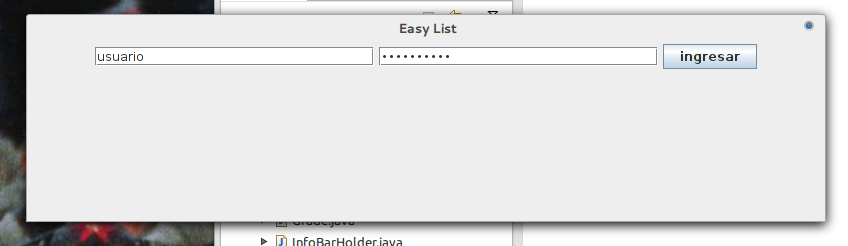
\includegraphics[width=0.85\textwidth]{figuras/ejemplo-a.png}
  \caption{EasyList pantalla inicial.}
  \label{fig:easylist-inicio}
\end{figure}

Esta segunda parte se denomino EasyList, y como se puede ver en la figura \ref{fig:easylist-inicio} permite elegir el nombre de usuario y contraseña con el cual se desea acceder a la base de datos. La ubicación de la base de datos y el proveedor de \dd que se usara deben especificarse en el código de la clase, por lo que si se pretende usar un motor o base diferente eso debe ser cambiado en el código fuente.
%

\begin{figure}[h]
  \centering
    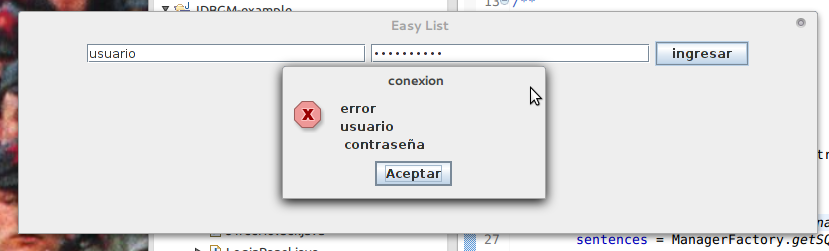
\includegraphics[width=0.85\textwidth]{figuras/ejemplo-b.png}
  \caption{Manejo de errores en EasyList}
  \label{fig:easylist-error}
\end{figure}
%

Como se puede ver en la figura \ref{fig:easylist-error} se incluyo un ejemplo de manejo de excepciones para la vista inicial de \textit{login}. Si se intenta acceder con un nombre de usuario y/o contraseña incorrecto \verb=ManagerFactory= lanzara una excepción pues no va a poder realizar la conexión con motor, por lo que es posible para EasyList capturar esta excepción e informarle a el usuario de la aplicación de dicho error\footnote{En este caso en el mensaje de error se muestra la contraseña en texto plano, algo que siempre debe evitarse por cuestiones de seguridad.} sin que el programa se cuelgue, o sea que el programa posee un modo de recuperarse de algunos errores.

\begin{figure}[h]
  \centering
    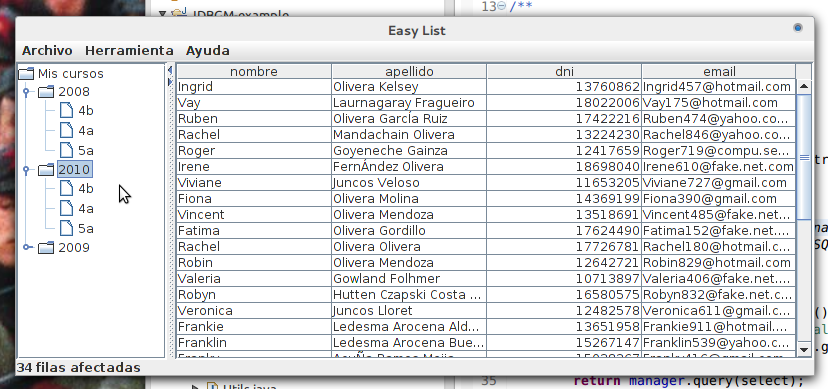
\includegraphics[width=0.85\textwidth]{figuras/ejemplo-c.png}
  \caption{Acceso correcto en EasyList}
  \label{fig:easylist}
\end{figure}

La figura \ref{fig:easylist} muestra como se ve EasyList cuando el usuario pudo ingresar satisfactoriamente sus datos de autenticación. El único elemento realmente funcional de esta interfaz es el árbol de la izquierda que muestra los años que fueron registrados, y por cada año los cursos que fueron registrados por el programa y por cada uno de estos cursos se muestra los alumnos que estaban matriculados en ellos. La lógica de todas estas consultas están contenidas en la clase \verb=DataObtainer= que es la encargada, como su nombre lo dice, de obtener todos los datos de la base de datos. Todas las otras clases que componen esta segunda aplicación son necesarias únicamente para crear la interfaz gráfica.

Al igual que en la aplicación anterior es necesario únicamente cambiar una linea de código para poder usar un \dd distinto. La elección de un motor distinto se podría haber echo dinámicamente  antes de que el usuario ingrese sus credenciales de acceso, pues como ya se menciono anteriormente basta con elegir una constante diferente para indicarle a \verb=ManagerFactory= que se desea usar un motor diferente\footnote{Suponiendo que la ubicación del motor elegido sea siempre la misma que la de los otros motores}, pero como se quería mantener lo más simple posible la aplicación de ejemplo esto no se implemento.

\section{Resumen}
La importancia de la aplicación de ejemplo es la de mostrar la facilidad con la que se puede migrar de un motor a otro cuando se usa \jj, es por ello que las dos partes que componen el ejemplo son tan simples. Además estas clases que se crearon sirven como guía básica, aparte del manual, para comprender como se usa la librería presentada en este proyecto.

Se puede encontrar todo el código de la aplicación de ejemplo en el repositorio publico \url{https://github.com/nerones/JDBGM-example} alojado en los servidores de \href{https://github.com/}{Github}\footnote{Github es un popular servicio que ofrece alojamiento gratuito para repositorios git que alojen proyectos \textit{open source}}.